\section{Data Details}
\label{supp:data}
\subsection{\molmoacttsodata Statistics}
\label{supp:so100-so101-stats}

We use \molmoacttsodata in the \molmoactt training mixture. We first collect 1{,}660 dataset entries; then we use TOPReward \citep{chen2026topreward} to filter out 438
low-quality dataset entries, yielding 1{,}222 final
datasets. All statistics below are computed only over this final filtered set. \Cref{tab:so100-so101-summary} presents the summary statistics for the SO-100/101 training partition. \Cref{tab:so100-so101-robot-type} presents the number of datasets by the type of SO-10x variants. \Cref{tab:so100-so101-metadata} presents the distribution of different metadata such as FPS, camera configuration, and action/state dimensions. \Cref{fig:action_verbs} presents the distribution of action verbs before and after the language annotation pipeline described in \Cref{sec:lang_annot}. \Cref{fig:so100_sample} shows several sample trajectories from the dataset partition. 
\begin{figure}[htb!]
    \centering
    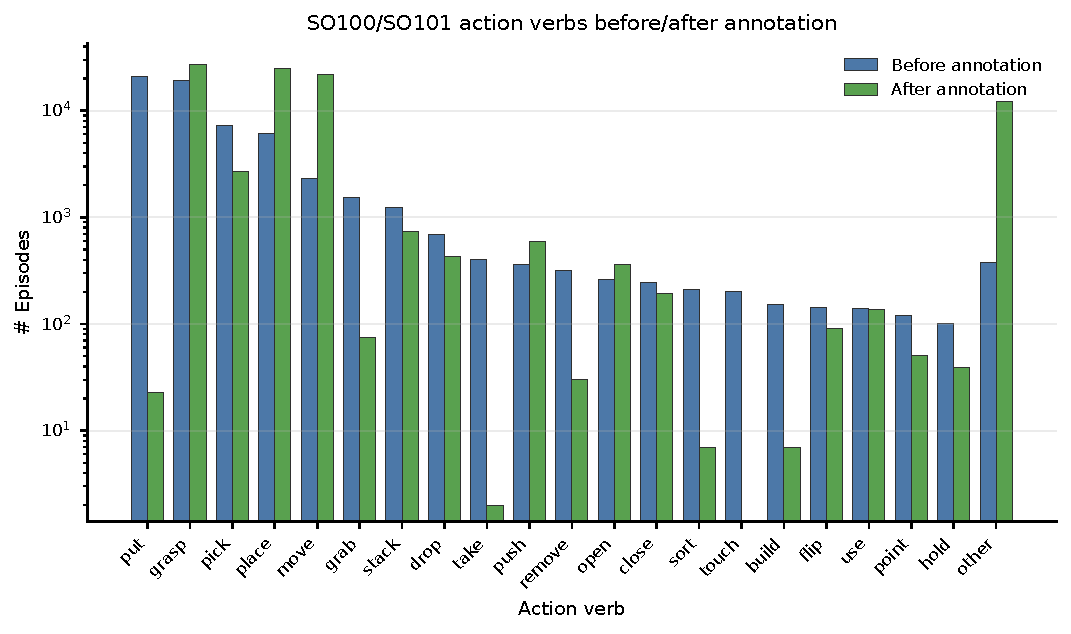
\includegraphics[width=0.9\linewidth]{figures/so100_annotation_before_after_action_verb_histogram.pdf}
    \caption{\textbf{Action verb distribution before and after language annotation.} }
    \label{fig:action_verbs}
\end{figure}

\begin{figure}[htb!]
    \centering
    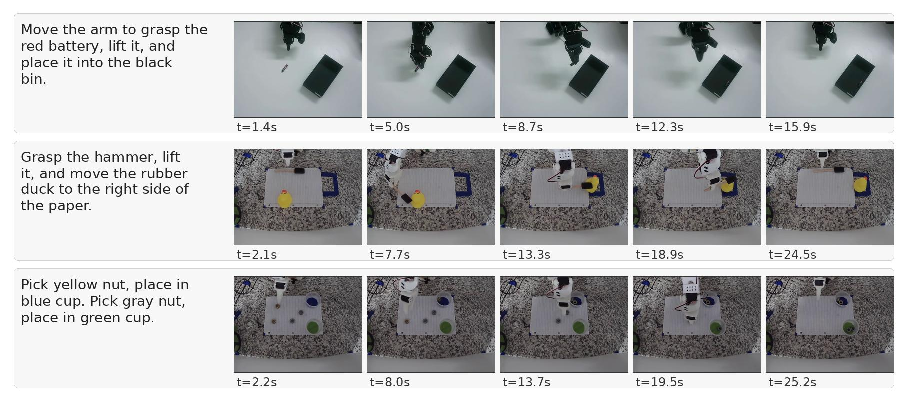
\includegraphics[width=0.9\linewidth]{figures/so100_sample_episode_frames.pdf}
    \caption{\textbf{Sample trajectories from the SO10x dataset partition.} }
    \label{fig:so100_sample}
\end{figure}


\begin{table}[ht]
\centering
\footnotesize
\caption{\textbf{Summary statistics for the SO-100/101 training subset.} We
report statistics for the final filtered \molmoacttsodata partition.}
\setlength{\tabcolsep}{6pt}
\renewcommand{\arraystretch}{1.1}
\begin{tabular}{lr}
% \toprule
\textbf{Statistic} & \textbf{Value} \\
\midrule
\# datasets & 1{,}222 \\
Contributors & 377 \\
Episodes & 38{,}059 \\
Frames & 19.8M \\
Estimated duration & 183.6 hours \\
Metadata task count & 1{,}322 \\
Instruction rows & 38{,}059 \\
Globally unique instructions & 12{,}818 \\
Unique-instruction ratio & 33.7\% \\
Datasets with annotated task metadata & 1{,}222 \\
% \bottomrule
\end{tabular}
\label{tab:so100-so101-summary}
\end{table}

\begin{table}[t]
\centering
\footnotesize
\caption{\textbf{SO-10x data partition breakdown by robot type.}}
\setlength{\tabcolsep}{5pt}
\renewcommand{\arraystretch}{1.1}
\begin{tabular}{lrrrr}
% \toprule
\textbf{Robot type} & \textbf{Datasets} & \textbf{Episodes} & \textbf{Frames} & \textbf{Hours} \\
\midrule
SO-100 & 921 & 31{,}101 & 15.18M & 141.7 \\
SO-101 & 299 & 6{,}898 & 4.57M & 41.6 \\
MOSS & 2 & 60 & 15.6K & 0.2 \\
% \bottomrule
\end{tabular}
\label{tab:so100-so101-robot-type}
\end{table}



\begin{table}[t]
\centering
\footnotesize
\caption{\textbf{Recording and feature metadata.} Most demonstrations are
recorded at 30 Hz with two camera streams; all final filtered datasets use
six-dimensional action and state vectors.}
\setlength{\tabcolsep}{6pt}
\renewcommand{\arraystretch}{1.1}
\begin{tabular}{lrrrr}
% \toprule
\textbf{Metadata field} & \textbf{Value} & \textbf{Datasets} & \textbf{Episodes} & \textbf{Frames} \\
\midrule
FPS & 30 & 1{,}114 & 36{,}828 & 18.96M \\
FPS & 20 & 78 & 527 & 261.4K \\
FPS & 25 & 18 & 423 & 256.7K \\
FPS & 60 & 8 & 208 & 231.6K \\
Camera count & 1 & 230 & 4{,}159 & 2.26M \\
Camera count & 2 & 835 & 24{,}151 & 13.05M \\
Camera count & 3 & 151 & 9{,}235 & 4.11M \\
Camera count & 4 & 6 & 514 & 342.1K \\
Action dimension & 6 & 1{,}222 & 38{,}059 & 19.76M \\
State dimension & 6 & 1{,}222 & 38{,}059 & 19.76M \\
% \bottomrule
\end{tabular}
\label{tab:so100-so101-metadata}
\end{table}

\subsection{Language Annotation Pipeline Implementation Details}
\label{supp:language-annotation-details}
Running inference with temperature 0.1 and max\_length set to 1024 tokens, we feed the following prompt into Qwen3.5-27B:
\begin{quote} 
You are an expert robot arm task instruction generator. You are provided with multiple demonstration videos, each showing the exact same task execution captured simultaneously from different camera angles. The task is to \{original\_instruction\}. Based on these videos, generate a clear imperative instruction describing all of the actions performed by the robot arm. Carefully study the evolution of the state of the scene, to understand how the robot arm achieves the goal. Pay attention to the color and position of the objects the robot interacts with. Start directly with an action verb and make sure you do not miss any actions. Note that the robot arm is not always grasping an object and maybe pushing objects around instead. Verify any grasps by checking the gripper state, and only say the arm is grasping an object if this is shown in the wrist camera when the gripper is closed. Your prompts should be almost exactly \{word\_limit\} words long.
\end{quote}

 word\_limit is a number randomly sampled from a right tailed power distribution, with a minimum value of 5 and a maximum value of 25. In addition to the text prompt, for each of the cameras in the trajectory that are not frozen, we sample 12 frames that are each equally temporally spaced and pass the frames to the model. 
 
 Running this pipeline results in the changes to the number of unique instructions in the datasets shown in Table \ref{tab:language-annot_increased}.

\begin{table}[t]
\centering
\footnotesize
\caption{\textbf{Dataset Language Annotation Diversity.} Running the language annotation pipeline increases the number of unique instructions for all of the robotics datasets in \molmoactt's training mix.}
\setlength{\tabcolsep}{5pt}
\renewcommand{\arraystretch}{1.1}
\begin{tabular}{lcc}
% \toprule
\textbf{Dataset} & \textbf{Original Instructions} & \textbf{Relabeled Instructions}\\
\midrule
\molmoacttyamdata & 34 (0.1\%)     & 11448 (35\%)   \\
\midrule
\molmoacttdroiddata            & 49623 (67\%)   & 55905 (75\%)   \\
\midrule
\molmoacttsodata            & 707 (1.5\%)    & 16205 (34\%)   \\
\midrule
\molmoactdata       & 134 (1\%)      & 2959 (28\%)    \\
\midrule
BC-Z             & 104 (0.3\%)    & 9981 (25\%)    \\
\midrule
Fractal          & 598 (0.7\%)    & 16729 (19\%)   \\
\midrule
Bridge           & 19973 (37\%)   & 35096 (66\%)   \\
\midrule
\textbf{Total}   & \textbf{71121 (22\%)} & \textbf{146485 (46\%)} \\
\end{tabular}
\label{tab:language-annot_increased}
\end{table}


% \subsection{Past tabletop bimanual manipulation datasets}
\begin{table}[t]
\centering
\footnotesize
\caption{\textbf{Past Tabletop Bimanual Manipulation Datasets.} \molmoacttyamdata is the largest open-source tabletop bimanual robotics dataset. In this table, we compare against other open and closed-source tabletop bimanual datasets from the literature.}
\setlength{\tabcolsep}{5pt}
\renewcommand{\arraystretch}{1.1}
\begin{tabular}{lccc}
\toprule
\textbf{Dataset Name} & \textbf{Embodiment} & \textbf{Number of Trajectories} & \textbf{Open / Closed?}\\
\midrule
{\color{ai2pink}\molmoacttyamdata (Ours)} & {\color{ai2pink}Bimanual YAM} & {\color{ai2pink}34,500} & {\color{ai2pink}Open}  \\ 
\midrule
AIST Bimanual Manipulation Dataset~\citep{motoda2025aistdata} & ALOHA & 10,000 & Open \\ 
\midrule
BiPlay Dataset~\citep{dasari2025ingredients} & ALOHA & 7,000 & Open \\ 
\midrule
RDT-1B Finetuning Dataset~\citep{liu2024rdt} & ALOHA & 6,000 & Open \\ 
\midrule
ALOHA Unleashed Training Data~\citep{zhao2024aloha} & ALOHA & 26,000 & Closed \\
\midrule
SARM RA-BC Dataset~\citep{chen2025sarm} & Bimanual YAM & 200 Hours & Closed \\ 
\bottomrule
\end{tabular}
\label{tab:past_robot_data}
\end{table}

% \begin{table}[t]
% \centering
% \footnotesize
% \caption{\textbf{Previous  open-source robotics manipulation datasets} TODO}
% \setlength{\tabcolsep}{5pt}
% \renewcommand{\arraystretch}{1.1}
% \begin{tabular}{l p{0.3\linewidth} c}
% % \toprule
% \textbf{Dataset Name} & \textbf{Embodiment} & \textbf{Number of Trajectories}\\
% \midrule
% AGIBot World~\citep{agibotworldcontributors2025agibotworldcolosseolargescale} & AGIBot & 1,000,000 \\ 
% \midrule
% RoboMIND 2.0~\citep{hou2025robomind} & Franka, Ur5E, AgileX, ARX, TienKung, TianYi & 310,000 \\ 
% \midrule
% RoboNet~\citep{dasari2019robonet} & Franka, WidowX, Sawyer, Baxter, Kuka, Fetch, Google Robot & 162,000 \\
% \midrule
% RH20T~\citep{fang2023rh20t} & Franka, Kuka, UR5, Flexiv & 110,000 \\
% \midrule
% Galaxea Open-World Dataset~\citep{jiang2025galaxea} & Galaxea R1 Lite & 100,000 \\ 
% % \bottomrule
% \end{tabular}
% \label{tab:past_robot_data}
% \end{table}
% \subsection{Action Reasoning Data}

% We construct the \emph{Action Reasoning Data} by converting conventional robot episodes $(I_t, L, A_t)$ into an augmented autoregressive sequence in which each timestep is supplemented with two additional supervisory signals: discretized depth tokens and a visual reasoning trace. Depth targets are obtained by inferring dense depth maps from RGB observations using DepthAnything-v2, followed by quantization with a VQ-VAE trained for 20~epochs on 10~million tabletop manipulation images, yielding an $h \times w$ grid of codebook indices that serve as the \textsc{DepthTokens}. The visual reasoning trace consists of a sequence of pixel coordinates representing the projected near-future motion of the end-effector, obtained by prompting a vision–language model to localize the gripper in each frame and selecting one to five points spanning from the current timestep to a designated future index. The resulting sequence for each timestep comprises the depth tokens, the visual reasoning trace, and the action vector (end-effector pose delta and gripper state), which are used jointly for autoregressive training with cross-entropy over discrete tokens and an $\ell_1$ loss over continuous action parameters. The final corpus contains 21{,}101{,}636 labeled frames, sourced from \textsc{BC-Z} (10{,}289{,}224; 48.8\%), \textsc{RT-1} (7{,}065{,}620; 33.5\%), and \textsc{Bridge-v2} (3{,}746{,}792; 17.8\%). Unless otherwise specified, mini-batches are sampled in proportion to these dataset shares to maintain source distribution during training. We defined the task, its description, the corresponding language instruction, and the task progression metric ratings.

% Ascii







% \subsection{\molmoactdata}

% \molmoactdata has two external camera views and a single wrist camera view. In the home environment data, the camera view configuration may vary between tasks, whereas for the tabletop data it remains the same for all tasks. For each task, we first rank the two external camera views based on scene clarity (i.e., how well the robot and objects are visible) and whether the view is occluded by the robot during task execution. Based on this ranking, we label them as the \textit{primary} and \textit{secondary} camera views. All home environment data is recorded at 15 Hz, while all tabletop data is recorded at 20 Hz. The tabletop data additionally includes extrinsic and intrinsic camera calibration matrices for both external cameras available on . We list details of the tasks we collected for \molmoact Dataset in Table \ref{tab:home_task} and \ref{tab:tabletop_task}. 


      
% \begin{table}[t]
% \centering
% \begingroup
% \setlength{\tabcolsep}{1pt}
% \setlength{\arrayrulewidth}{0.1pt}
% \renewcommand{\arraystretch}{1.1}
% \scriptsize
% \begin{tabular}{|p{0.11\linewidth}|p{0.26\linewidth}|p{0.34\linewidth}|p{0.25\linewidth}|}
% \hline
% \textbf{Scene} & \textbf{Task} & \textbf{Language Instruction} & \textbf{Object(s)} \\
% \hline
% \csvreader[
%   separator=comma,
%   head to column names,
%   late after line=\\\hline
% ]{\detokenize{tables/appendix/MolmoAct_Dataset_home.csv}}{}%
% {\csvcoliii & \texttt{\csvcoli} & \csvcolii & \csvcoliv}
% \end{tabular}
% \caption{Tasks details of \molmoactdata Home Environemnt including scene, task name, language instruction and all objects used for data collection.}
% \label{tab:home_task}
% \endgroup
% \end{table}



% \begin{table}[t]
% \centering
% \begingroup
% \setlength{\tabcolsep}{1pt}
% \setlength{\arrayrulewidth}{0.1pt}
% \renewcommand{\arraystretch}{1.1}
% \scriptsize
% \begin{tabular}{|p{0.11\linewidth}|p{0.26\linewidth}|p{0.34\linewidth}|p{0.25\linewidth}|}
% \hline
% \textbf{Scene} & \textbf{Task} & \textbf{Language Instruction} & \textbf{Object(s)} \\
% \hline
% \csvreader[
%   separator=comma,
%   head to column names,
%   late after line=\\\hline
% ]{\detokenize{tables/appendix/MolmoAct_Dataset_tabletop.csv}}{}%
% {\csvcoliii & \texttt{\csvcoli} & \csvcolii & \csvcoliv}
% \end{tabular}
% \caption{Tasks details of \molmoactdata Tabletop Environemnt including scene, task name, language instruction and all objects used for data collection.}
% \label{tab:tabletop_task}
% \endgroup
% \end{table}



% \begin{table}[t]
% \centering
% \begingroup
% \setlength{\tabcolsep}{2pt}        % was 4pt; tighter padding, same column widths
% \setlength{\arrayrulewidth}{0.3pt} % slightly thinner vertical lines
% \renewcommand{\arraystretch}{1.1}
% \scriptsize
% \begin{tabular}{|p{0.08\linewidth}|p{0.26\linewidth}|p{0.34\linewidth}|p{0.28\linewidth}|}
% \hline
% \textbf{Scene} & \textbf{Task} & \textbf{Language Instruction} & \textbf{Object(s)} \\
% \hline
% \csvreader[
%   separator=comma,
%   head to column names,
%   late after line=\\\hline
% ]{figures/Molmo-ACT_Dataset.csv}{}%
% {\csvcoliii & \texttt{\csvcoli} & \csvcolii & \csvcoliv}
% \end{tabular}
% \caption{Prompts from \texttt{figures/Molmo-ACT_Dataset.csv} grouped by scene order.}
% \label{tab:molmoact_task_detail}
% \endgroup
% \end{table}
